\documentclass{../../assignment}
\usepackage{amsmath}
\usepackage{graphicx}
\usepackage{subfigure}
\usepackage{hyperref}
\usepackage{listings}
\usepackage{float}
\lstset{numbers=left}

\coursetitle{Computer Vision II}
\courselabel{CSE 252B}
\exercisesheet{Homework 4}{}
\student{Zhu, Zhongjian}
\university{University of California, San Diego}
\semester{Winter 2017}
\date{\today}

\begin{document}
\begin{problemlist}

\pbitem Automatic estimation of the planar projective transformation
\begin{enumerate}
\item \textbf{Feature detection}\\
Calculate an image where each pixel value is the minor eigenvalue of the gradient matrix. Calculate the gradient images using the five-point central difference operator. Set resulting values that are below a specified threshold value to zero. Apply an operation that suppresses local nonmaximum pixel values in the minor eigenvalue image. Determine the subpixel feature coordinate.
\\\\
\textbf{Solution}\\
First, in order to get the gradient matrix, we need to filter the image in x- and y-direction. The convolution kernel is $\mathbf{k} = (-1,8,0,-8,1)^{\top}/12$. So the x-derivative image, $I_x$, is to filter each row with $\mathbf{k}^{\top}$ and the y-derivative image, $I_y$, is to filter each column with $\mathbf{k}$.

Then use the following equation to get the minor eigenvalue for each pixel.
\[
\mathbf{N} = 
\begin{bmatrix}
\sum_w I_x^2 &  \sum_w I_x I_y\\
\sum_w I_x I_y & \sum_w I_y^2
\end{bmatrix}.
\]

$$\lambda_{min} = \frac{Tr(\mathbf{N} - \sqrt{Tr(\mathbf{N})^2 - 4det(\mathbf{N})})}{2}$$
where $w$ is the window about the pixel, and $I_x$ and $I_y$ are the gradient images in the x and y direction, respectively. Set resulting values that are below a specified threshold value to zero. Now we get the minor eigenvalue matrix.

Next step is to apply the non-maxium suppression. For each pixel, we set a window on it and calculate the maximum value in the window, the local maximum. If the value of the center pixel of the window is less than the local maximum, set it to 0, otherwise, keep the value. This step is actually to find the corner pixels and set the value of non-corner pixels to 0.

Since what we need is not the corner pixel but rather the corner coordinates, we need to use the $\mathrm{F\ddot{o}stner}$ corner point operator to find the subpixels.
\[
\begin{bmatrix}
\sum_w I_x^2 &  \sum_w I_x I_y\\
\sum_w I_x I_y & \sum_w I_y^2
\end{bmatrix}
\begin{bmatrix}
x_{corner}\\
y_{corner}
\end{bmatrix}
=
\begin{bmatrix}
\sum_w (x I_x^2 + y I_x I_y\\
\sum_w (x I_x I_y + y I_y^2
\end{bmatrix}
\]
$x_{corner}$ and $y_{corner}$ are the coordinates of the subpixel.
\\\\
\textbf{Result}\\
The size of the feature detection window is $9\times9$, 
the minor eigenvalue threshold value is 6.5, 
the size of the local non-maximum suppression window is $9\times9$.\\
The number of features detected in \emph{price\_ center20.JPG} is 644, and the number of features detected in \emph{price\_ center21.JPG} is 642.
\begin{figure}[H]
\subfigure[]{
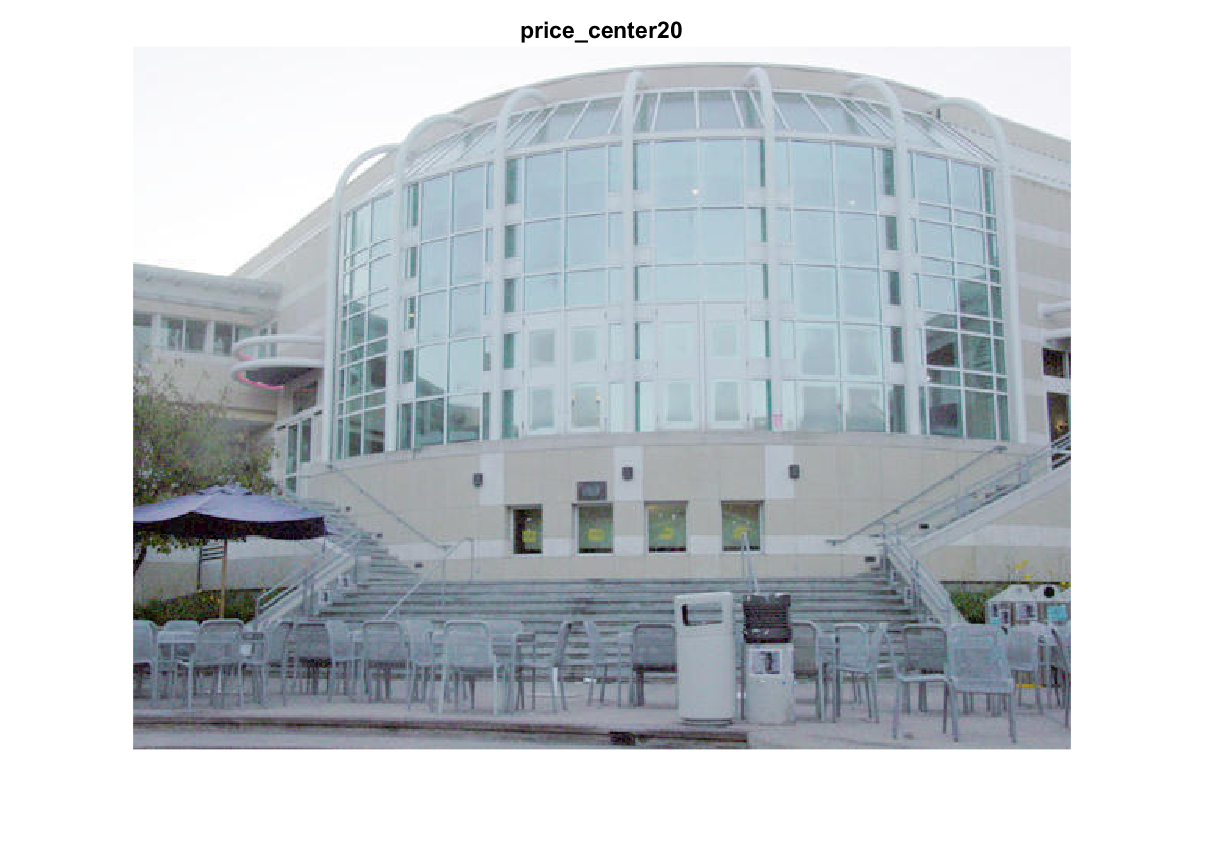
\includegraphics[width=0.5\textwidth]{PriceCenter_20}  
}
\subfigure[]{
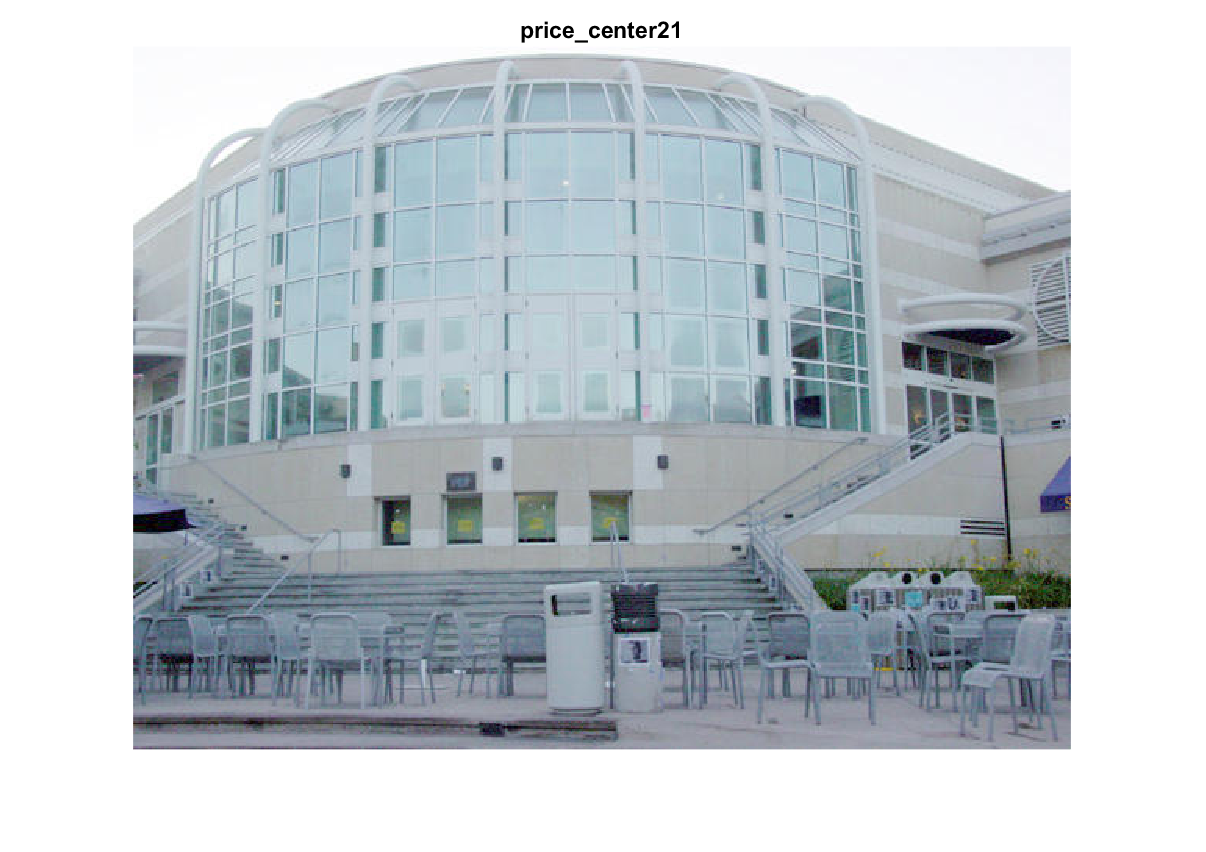
\includegraphics[width=0.5\textwidth]{PriceCenter_21}  
}
\caption{Input images. (a) price\_center20. (b) price\_center21.}
\label{fig:images}
\end{figure}
 
\begin{figure}[H]
\subfigure[]{
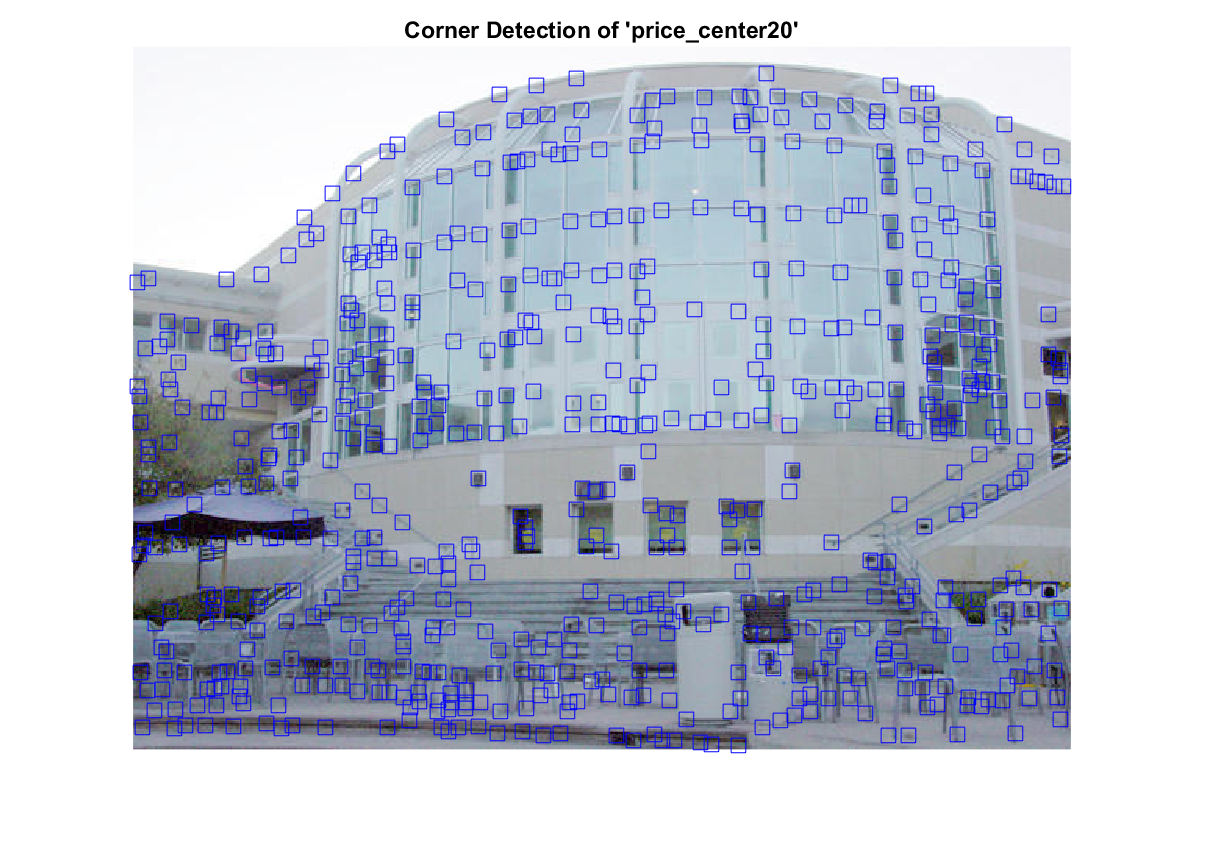
\includegraphics[width=0.5\textwidth]{CornerDetection_20}
}
\subfigure[]{
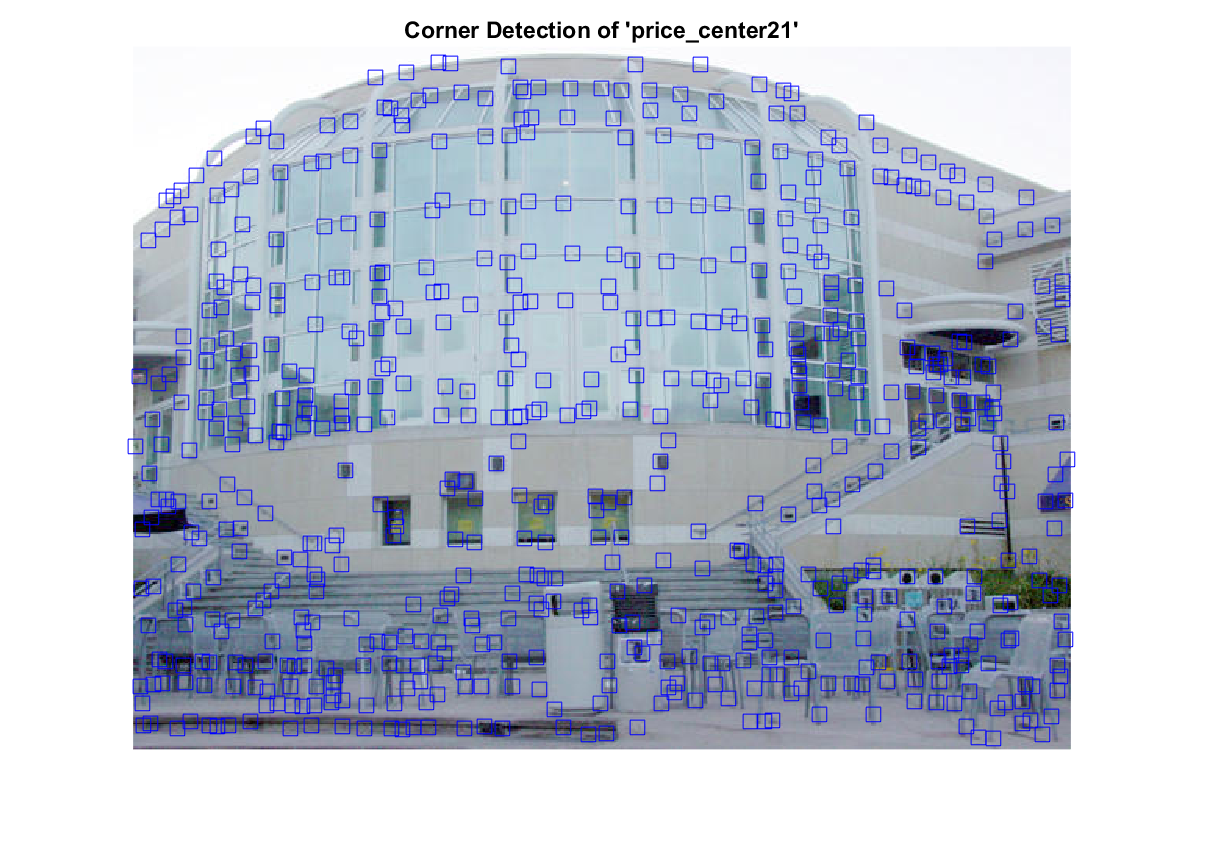
\includegraphics[width=0.5\textwidth]{CornerDetection_21}  
}
\caption{Detected corners. (a) price\_center20. (b) price\_center21.}
\label{fig:images}
\end{figure} 



\item \textbf{Feature matching}\\
Determine the set of one-to-one putative feature correspondences by performing a brute-force search for the greatest correlation coefficient value between windows centered about the detected features in image 1 and windows centered about the detected features in image 2. Only allow matches that are above a specified correlation coefficient threshold value. Further, only allow matches that are above a specified distance ratio threshold value, where distance is measured to the next best match for a given feature. Vary these parameters such that around 200 putative feature correspondences are established. Optional: constrain the search to coordinates in image 2 that are within a proximity of the detected feature coordinates in image 1.
\\\\
\textbf{Solution}\\
First we need to calculate the correlation coefficient between a given window in image 1 and all windows in image 2. Here since the subpixel value do not exist in image coordinate, we need to use interpolation.

Once we have the correlation matrix, we need to do the one-to-one matching. The algorithm is as follow:
\begin{lstlisting}
Find indices of element with maximum value
  If similarity threshold < maximum value
    Store the best match value
    Set element to -1
    Find next best match value as
    max(next best match value in row, next best match value in column)    
    If (1-best match value)<(1-next best match value)*distance ratio threshold
      Store feature value
    else
      Match is not unique enough    
    Set row and column to -1
\end{lstlisting}


\textbf{Result}\\
The size of the proximity window is $25\times160$, the size of the matching window is $9\times9$, the correlation coefficient threshold value is 0.7, the distance ratio threshold value is 0.9, and the resulting number of putative feature correspondences is 217.\\
\begin{figure}[H]
\subfigure[]{
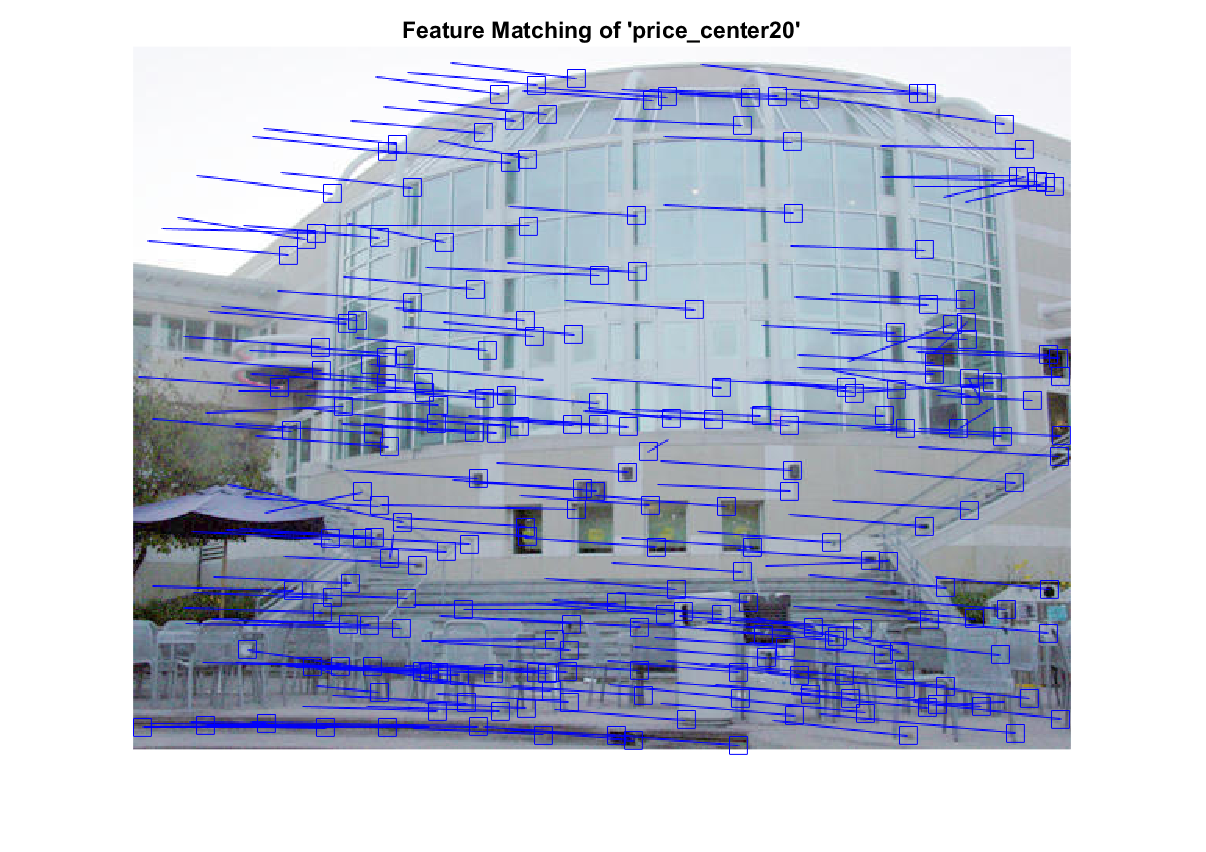
\includegraphics[width=0.5\textwidth]{FeatureMatch_20}  
}
\subfigure[]{
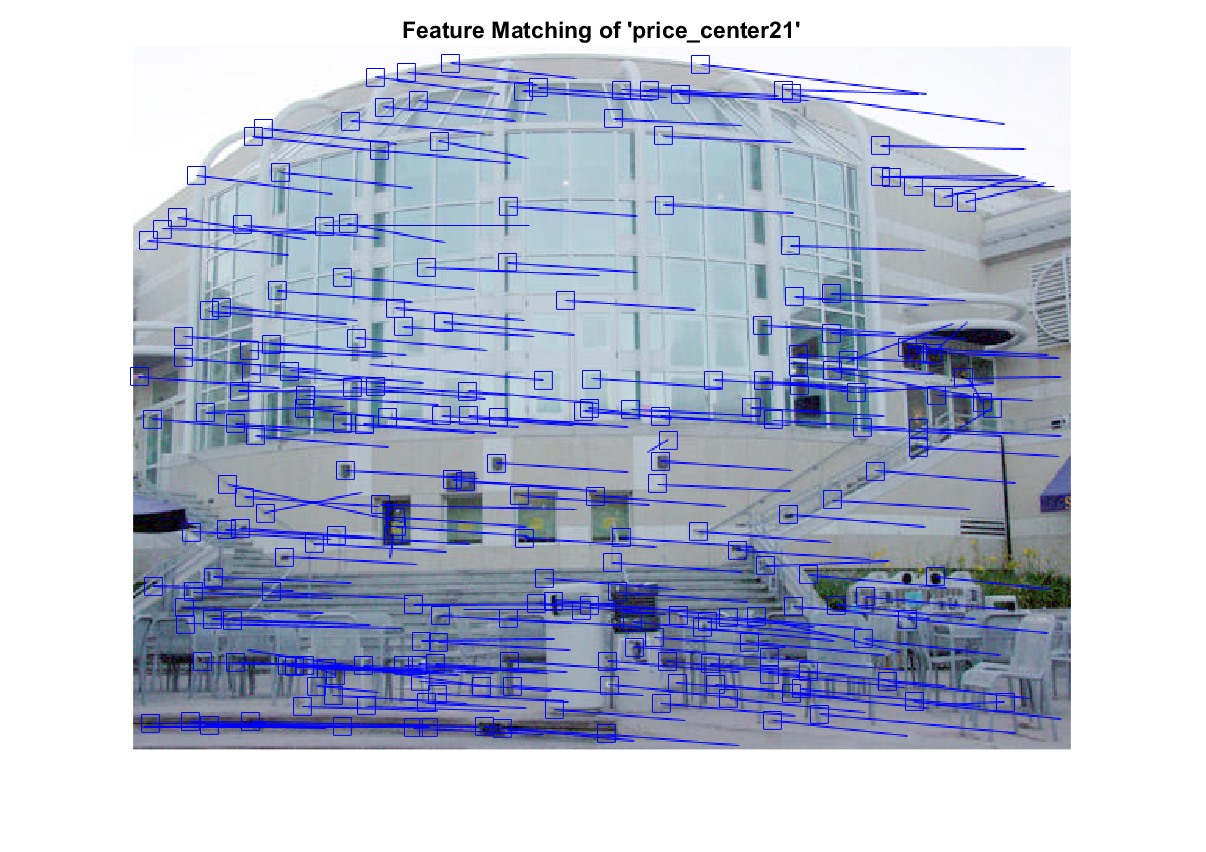
\includegraphics[width=0.5\textwidth]{FeatureMatch_21}  
}
\caption{Matched features. (a) price\_center20. (b) price\_center21.}
\label{fig:images}
\end{figure} 

\item \textbf{Outlier rejection}\\
The resulting set of putative point correspondences contain both inlier and outlier correspondences. Determine the set of inlier point correspondences using the M-estimator Sample Consensus (MSAC) algorithm, where the maximum number of attempts to find a consensus set is determined adaptively. Use the 4-point algorithm to estimate the planar projective transformation from the 2D points in image 1 to the 2D points in image 2. Calculate the Sampson error as a first order approximation to the geometric error.
\\\\
\textbf{Solution}\\
The adaptive number of trials MSAC algorithm can be concluded as follow:
\begin{lstlisting}
consensus_min_cost = inf
max_trials = inf
for(trials=0;trials<max_trials && consensus_min_cost>threshold;++trials)
{
  select a random sample
  calculate the model
  calculate the error
  calculate the cost
  if(consensus_min_cost<consensus_min_cost)
  {
    consensus_min_cost = consensus_cost
    consensus_min_cost_model = model
    number of inliers
    w = # of inliers / # of data points
    max_trials = log(1-p) / log(1-w^s)
  }
}
\end{lstlisting}
To calculate the model, $\mathbf{H}$, we need to use the canonical projective matrix:
\[
\mathbf{e}_1 = 
\begin{bmatrix}
1\\
0\\
0
\end{bmatrix}
\mathbf{e}_2 = 
\begin{bmatrix}
0\\
1\\
0
\end{bmatrix}
\mathbf{e}_3 = 
\begin{bmatrix}
0\\
0\\
1
\end{bmatrix}
\mathbf{e}_4 = 
\begin{bmatrix}
1\\
1\\
1
\end{bmatrix}
\]
The projection matrices from canonical basis to image 1 and image 2 are $\mathbf{H}_1$ and $\mathbf{H}_2$ respectively. So the projection matrix from image 1 to image 2 is $\mathbf{H} = \mathbf{H}_2^{-1}\mathbf{H}_1$.

To calculate the 2D projective transformation, 4 points are needed.
\[
\begin{bmatrix}
\mathbf{e}_1 & \mathbf{e}_2 & \mathbf{e}_3 & \mathbf{e}_4
\end{bmatrix} = 
\mathbf{H}
\begin{bmatrix}
s_1\mathbf{x}_1 & s_2\mathbf{x}_2 & s_3\mathbf{x}_3 & s_4\mathbf{x}_4
\end{bmatrix} = 
\mathbf{H}
\begin{bmatrix}
\lambda_1\mathbf{x}_1 & \lambda_2\mathbf{x}_2 & \lambda_3\mathbf{x}_3 & \mathbf{x}_4
\end{bmatrix}
\]
where $\lambda_i = s_i/s_4$. Since $\mathbf{H}$ is up-to-scale, this will lead to the same result.

\[
\begin{bmatrix}
\mathbf{e}_1 & \mathbf{e}_2 & \mathbf{e}_3
\end{bmatrix} = 
\mathbf{H}
\begin{bmatrix}
\lambda_1\mathbf{x}_1 & \lambda_2\mathbf{x}_2 & \lambda_3\mathbf{x}_3
\end{bmatrix} \mathrm{and}
\mathbf{e}_4 = \mathbf{H}\mathbf{x}_4
\]
So we can use
\[
\begin{bmatrix}
\mathbf{x}_1 & \mathbf{x}_2 & \mathbf{x}_3
\end{bmatrix}
\begin{bmatrix}
\lambda_1\\
\lambda_2\\
\lambda_3
\end{bmatrix}
 = 
\mathbf{x}_4
\]

to solve for $\mathbf{\lambda}$ and then use
\[
\mathbf{H}^{-1} = 
\begin{bmatrix}
\lambda_1\mathbf{x}_1 & \lambda_2\mathbf{x}_2 & \lambda_3\mathbf{x}_3
\end{bmatrix}
\]
to get $\mathbf{H}$.\\
The error used here is the Sampson error which is the first order approximation of thee geometric error.
$$\mathbf{\delta_X = -J^{\top}(JJ^{\top})^{-1}\epsilon}$$
where 
$$\mathbf{J} = \frac{\partial C_{\mathbf{H}}(\mathbf{X})}{\partial \mathbf{X}} = 
\begin{bmatrix}
-h_{21}+\tilde{y}'h_{31} & -h_{22}+\tilde{y}'h_{32} & 0 & \tilde{x}h_{32}+\tilde{y}h_{32}+h_{33}\\
h_{11}-\tilde{x}'h_{31} & h_{12}-\tilde{x}'h_{32} & -(\tilde{x}h_{31}+\tilde{y}h_{32}+h_{33}) & 0
\end{bmatrix}
$$
and
$$\epsilon = C_{\mathbf{H}}(\mathbf{X}) = 
\begin{bmatrix}
-(\tilde{x}h_{21}+\tilde{y}h_{22}+h_{23})+\tilde{y}'(\tilde{x}h_{31}+\tilde{y}'h_{32}+h_{33})\\
\tilde{x}h_{11}+\tilde{y}h_{12}+h_{13}-\tilde{x}'(\tilde{x}h_{31}+\tilde{y}'h_{32}+h_{33})
\end{bmatrix}
$$ 
is the cost associated with $\mathbf{X}$. So the Sampson error is $\|\delta_{\mathbf{X}}\|^2 = \epsilon^{\top}(\mathbf{JJ^{\top}})^{-1}\epsilon$.\\
Next step is to calculate the cost. First we set a tolerance. Here we use $t^2 = F_m^{-1}(\alpha)$ where $t^2$ is the mean squared distance threshold and $F_m^{-1}(\alpha)$ is the inverse chi-squared cumulative distribution function. We assume the probability that a data point is an inlier is 0.95, $\alpha = 0.95$, and the variance of the measurement error is 1, $\sigma^2 = 1$. The codimension $m = 2$. For points whose error is less or equal to the tolerance, we add the error to the cost and for those whose error is greater than the tolerance, we add the tolerance to the cost. The points whose error are less or equal to the tolerance are inliers and the others are outliers. Then if the cost is less than the previous cost, we keep the cost, the camera pose and the number of inliers. Then update the maximum number of trials.
\\\\
\textbf{Result}\\
The total number of the inliers are dependent on the choose of the points used to calculate the model, so we will have different number of inliers at each trial. Here we assumed that the probability $p$ that at least one of the random samples does not contain any outliers is 0.99, the probability $\alpha$ that a given data point is an inlier is 0.95 and the variance $\sigma^2$ of the measurement error is 1. In the code file, I keep one random seed which leads to 165 inliers. The number of maximum trials is 7.9519, so it runs 8 times to find the consensus set.
\begin{figure}[H]
\subfigure[]{
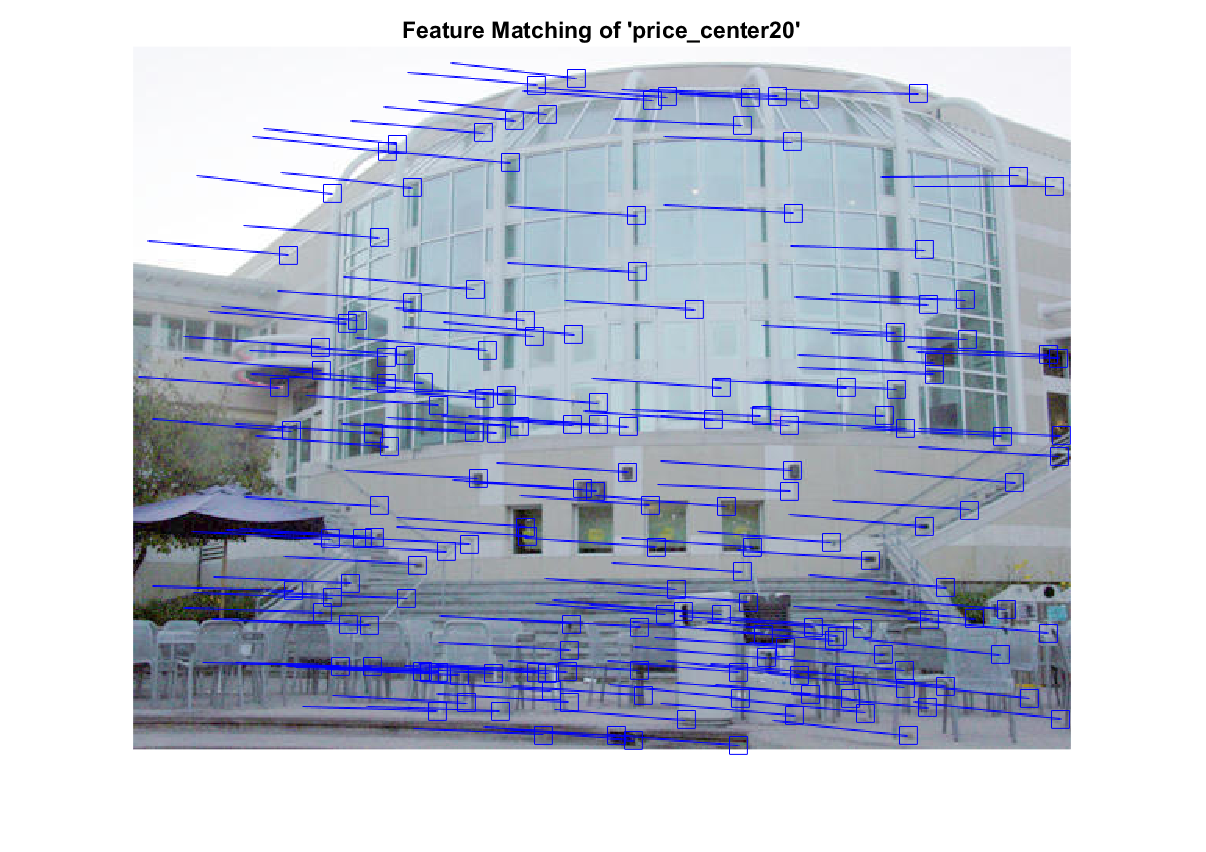
\includegraphics[width=0.5\textwidth]{FeatureMatch_20_inlier}  
}
\subfigure[]{
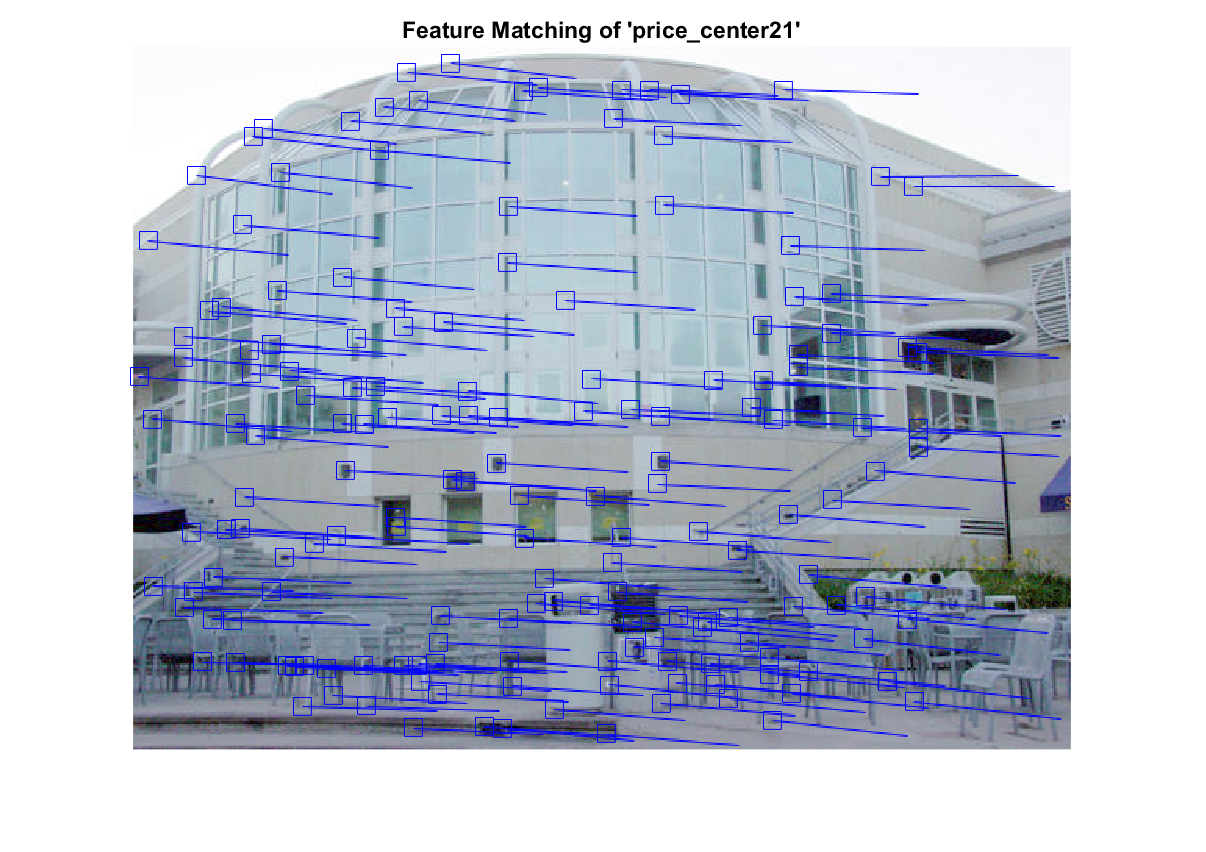
\includegraphics[width=0.5\textwidth]{FeatureMatch_21_inlier}  
}
\caption{Matched features of inliers. (a) price\_center20. (b) price\_center21.}
\label{fig:images}
\end{figure} 

\item \textbf{Linear estimation}\\
Estimate the planar projective transformation $\mathbf{H}_{DLT}$ from the resulting set of inlier correspondences using the direct linear transformation (DLT) algorithm (with data normalization).
\\\\
\textbf{Solution}\\
For DLT algorithm, we need first normalize data point by
$$
\mathbf{x}=
\begin{bmatrix}
s & 0 & -\mu_{\tilde{\mathbf{x}}}s\\
0 & s & -\mu_{\tilde{\mathbf{y}}}s\\
0 & 0 & 1
\end{bmatrix}\mathbf{x}
$$
where
$$
\sigma^2 = \sigma_{\tilde{\mathbf{x}}}^2 + \sigma_{\tilde{\mathbf{x}}}^2,
s = \frac{\sqrt{2}}{\sigma}
$$
Then we need to solve the equation below:
\[
\begin{bmatrix}
[\mathbf{x}'_1]^{\bot} \otimes \mathbf{x}_1^{\top}\\
[\mathbf{x}'_2]^{\bot} \otimes \mathbf{x}_2^{\top}\\
\vdots \\
[\mathbf{x}'_n]^{\bot} \otimes \mathbf{x}_n^{\top}\\
\end{bmatrix}\mathbf{h}=\mathbf{0}
\]
where $[\mathbf{x}_i]^{\bot}$ is the left null space of $\mathbf{x_i}$.
To get the left null space of $\mathbf{x_i}$, we need the Householder Matrix.
$$\mathbf{H_V} = \mathbf{I} - 2\frac{\mathbf{V V^{\top}}}{\mathbf{V^{\top} V}}$$
$$\mathbf{V} = \mathbf{x} + sign(x_1)\|\mathbf{x}\|\mathbf{e_1}$$
The 2 to 3 rows of $\mathbf{H_V}$ is the left null space of $\mathbf{x_i}$.\\
Since the DoF of $\mathbf{h}$ is 8, we need at least 4 points to solve the equation. Suppose the left null space is $\mathbf{A}$, using Singular Value Decomposition we can get
$$\mathbf{A} = \mathbf{U}\mathbf{\Sigma}\mathbf{V}^{\top}$$
and $\mathbf{h}$ is the last column of $\mathbf{V}$. Finally, reshape $\mathbf{h}$ to a $3\times 3$ matrix, denormalize it and divide it by its norm.
\\\\
\textbf{Result}\\
\[
\mathbf{H}_{DLT} = 
\begin{bmatrix}
0.0109600331801354  &  -2.00096871346898\times 10^{-5} & -0.984084957989864\\
0.000324711572734466 & 0.0106646222405988 & -0.176745394736336\\
1.26050707974689 \times 10^{-6} &  1.1124241298911\times 10^{-7} & 0.0101930644629375
\end{bmatrix}.
\]
\\
\item \textbf{Nonlinear estimation}\\
Use $\mathbf{H}_{DLT}$ and the Sampson corrected points as an initial estimate to an iterative estimation method, specifically the sparse Levenberg-Marquardt algorithm, to determine the Maximum Likelihood estimate of the planar projective transformation that minimizes the reprojection error.
\\\\
\textbf{Solution}\\
We first assume scene points $\mathbf{x}$ and then $\mathbf{x}' = \mathbf{H'x}$ and $\mathbf{x}'' = \mathbf{H''x}$. Furthermore, we assume $\mathbf{H' = I}$. As a result, we only need to calculate $\mathbf{H''}$. So for Levenberg-Marquardt algorithm, the parameter vector is $(\hat{\mathbf{h}}^{''\top},\hat{\tilde{\mathbf{x}}}_1^{\top},\hat{\tilde{\mathbf{x}}}_2^{\top},...,,\hat{\tilde{\mathbf{x}}}_n^{\top})^{\top}$, $\hat{\mathbf{h}}''$ is the parameterized $\mathbf{H}''$ and $\hat{\tilde{\mathbf{x}}}_i$ is the parameterized scene points.
The measurement vector is 
$(\hat{\tilde{\mathbf{x}}}_1^{'\top},\hat{\tilde{\mathbf{x}}}_2^{'\top},...,,\hat{\tilde{\mathbf{x}}}_n^{'\top},\hat{\tilde{\mathbf{x}}}_1^{''\top},\hat{\tilde{\mathbf{x}}}_2^{''\top},...,,\hat{\tilde{\mathbf{x}}}_n^{''\top})^{\top}$. The cost is $\epsilon^{'\top}\Sigma_{\mathbf{x}'}^{-1}\epsilon' + \epsilon''\Sigma_{\mathbf{x}''}^{-1}\epsilon''$. We assume $\Sigma_{\mathbf{x}_i}$ is an identity matrix.\\
For Jacobian matrix, here it is very sparse, so there is no need to calculate the full matrix. We only need to calculate three terms:
$$
\begin{matrix}
\mathbf{A}''_i = \frac{\partial \hat{\tilde{\mathbf{x}}}''_i}{\partial \hat{\mathbf{h}}''} & 
\mathbf{B}'_i = \frac{\partial \hat{\tilde{\mathbf{x}}}'_i}{\partial \hat{\tilde{\mathbf{x}}}} & 
\mathbf{B}''_i = \frac{\partial \hat{\tilde{\mathbf{x}}}''_i}{\partial \hat{\tilde{\mathbf{x}}}}
\end{matrix}.
$$
For normal equations matrix,$\mathbf{J}^{\top}\Sigma_{\mathbf{x}}^{-1}\mathbf{J}$ we still only need to calculate three terms:
$$
\begin{matrix}
\mathbf{U}'' = \sum_i \mathbf{A}_i^{''\top}\Sigma_{\mathbf{x}''_i}^{-1}  \mathbf{A}_i^{''} 
& 
\mathbf{V}_i = \mathbf{B}_i^{'\top}\Sigma_{\mathbf{x}'_i}^{-1}  \mathbf{B}_i^{'} + \mathbf{B}_i^{''\top}\Sigma_{\mathbf{x}''_i}^{-1}  \mathbf{B}_i^{''}
& 
\mathbf{W}_i'' = \mathbf{A}_i^{''\top}\Sigma_{\mathbf{x}''_i}^{-1}  \mathbf{B}_i^{''} 
\end{matrix}.
$$
The normal equations vector is $(\epsilon_{\mathbf{h}''}^{\top},\epsilon_{\hat{\tilde{\mathbf{x}}}_1}^{\top},\epsilon_{\hat{\tilde{\mathbf{x}}}_2}^{\top},...,\epsilon_{\hat{\tilde{\mathbf{x}}}_n})^{\top}$
where
$$
\begin{matrix}
\epsilon_{\mathbf{h}''} = \sum_i \mathbf{A}_i^{''\top}\Sigma_{\mathbf{x}_i}^{-1}  \epsilon''_i
&
\epsilon_{\hat{\tilde{\mathbf{x}}}_i} = \mathbf{B}_i^{'\top}\Sigma_{\mathbf{x}'_i}^{-1}  \epsilon'_i + \mathbf{B}_i^{''\top}\Sigma_{\mathbf{x}''_i}^{-1}  \epsilon''_i
\end{matrix}.
$$
The augmented normal equations are
$$
\mathbf{S}''=\mathbf{U''+\lambda I}-\sum_i \mathbf{W}_i^{''\top}(\mathbf{V}_i+\lambda \mathbf{I})^{\top}\mathbf{W}_i^{''\top}
$$
$$
\mathbf{e}''= \epsilon_{\mathbf{h}''} - \sum_i \mathbf{W}_i^{''\top}(\mathbf{V}_i+\lambda \mathbf{I})^{-1} \epsilon_{\hat{\tilde{\mathbf{x}}}_i}
$$
So we can get $\delta_{\mathbf{h}''}$ by solving $\mathbf{S}''\delta_{\mathbf{h}''} = \mathbf{e}''$ and then $\delta_{\hat{\tilde{\mathbf{x}}}_i} = (\mathbf{V}_i+\lambda \mathbf{I})^{-1}(\epsilon_{\hat{\tilde{\mathbf{x}}}_i} - \mathbf{W}_i^{''\top}\delta_{\mathbf{h}''})$. Add these two to the parameter vector to get the new parameter vector. Deparameterize the parameter vector and project the scene points to image 1 and image 2. Calculate the current cost and compare it the with previous cost. If the current cost is less than the previous cost, keep the parameter vector and error vector and set $\lambda = 0.1\lambda$. Iteration until the difference of cost between two iterations is less than 0.0001.
\\\\
\textbf{Result}\\
The costs of each iteration are as follow:
\begin{center}  
\begin{tabular}{|l|l|}
\hline
Iteration&Cost\\
\hline
0&59.0808\\
\hline 
1&58.8801\\
\hline 
2&58.8413\\
\hline
3&58.8413\\
\hline  
\end{tabular}
\end{center}
The $\mathbf{H}_{LM}$ is
\[
\mathbf{H}_{LM} = 
\begin{bmatrix}
0.0109600116108005  &  -2.11106791008192\times 10^{-5} & -0.983949182484355\\
0.000329426569889086 & 0.0106594313943083 & -0.177500139570516\\
1.27286063438928\times 10^{-6} &  9.85386977683278\times 10^{-7} & 0.0101908017104713
\end{bmatrix}.
\]

\end{enumerate}
\end{problemlist}

\begin{flushleft}
\large{\textbf{Appendix}}
\end{flushleft}

\lstinputlisting[language=MATLAB, caption = Part(a)]{../src/Q1.m}
\lstinputlisting[language=MATLAB, caption = Part(b)]{../src/Q2.m}
\lstinputlisting[language=MATLAB, caption = Part(c)]{../src/Q3.m}
\lstinputlisting[language=MATLAB, caption = Part(d)]{../src/Q4.m}
\lstinputlisting[language=MATLAB, caption = Part(e)]{../src/Q5.m}

\lstinputlisting[language=MATLAB, caption = Function]{../src/CornerCoordinate.m}
\lstinputlisting[language=MATLAB, caption = Function]{../src/FeatureMatch.m}
\lstinputlisting[language=MATLAB, caption = Function]{../src/parameterization.m}
\lstinputlisting[language=MATLAB, caption = Function]{../src/deparameterization.m}

\lstinputlisting[language=MATLAB, caption = Function]{../src/jcbA.m}
\lstinputlisting[language=MATLAB, caption = Function]{../src/jcbB1.m}
\lstinputlisting[language=MATLAB, caption = Function]{../src/jcbB2.m}
\lstinputlisting[language=MATLAB, caption = Function]{../src/jcb.m}

\lstinputlisting[language=MATLAB, caption = Function]{../src/SampsonError.m}
\lstinputlisting[language=MATLAB, caption = Function]{../src/NormalEquationsMatrix.m}
\lstinputlisting[language=MATLAB, caption = Function]{../src/NormalEquationsVector.m}
\lstinputlisting[language=MATLAB, caption = Function]{../src/AugmentedNormalEquations.m}

\end{document}
